\subsubsection{Casos d’ús principals}

Mentre que els requisits funcionals descrits anteriorment defineixen les capacitats que ha de proporcionar el sistema, els casos d’ús següents mostren com aquestes capacitats s’apliquen des de la perspectiva dels actors principals. En tots els casos, l’usuari continua mantenint la decisió final sobre la confirmació o cancel·lació de l’operació.

La Taula~\ref{tab:casos_us} resumeix els casos d’ús considerats en la proposta.

\begin{table}[H]
\centering
\small
\renewcommand{\arraystretch}{1.25}
\begin{tabularx}{\textwidth}{p{0.23\textwidth} p{0.18\textwidth} X}
\hline
\textbf{Cas d’ús} & \textbf{Actor} & \textbf{Descripció} \\
\textbf{} & \textbf{principal} & \textbf{} \\
\hline

CU1 -- Anàlisi prèvia d’una transacció &
Usuari &
L’usuari inicia una operació des d’una DApp o una interfície externa compatible. MetaMask rep la transacció, activa el Snap i mostra el resultat de l’anàlisi abans de la confirmació. \\

CU2 -- Anàlisi d’una aprovació ERC20 &
Usuari &
L’usuari intenta autoritzar una adreça per operar amb tokens fungibles. El sistema interpreta l’operació \texttt{approve} i diferencia entre revocacions, aprovacions limitades i aprovacions molt elevades o pràcticament il·limitades. \\

CU3 -- Anàlisi d’un permís global NFT &
Usuari &
L’usuari intenta executar una operació \texttt{setApprovalForAll} sobre una col·lecció NFT. El sistema detecta si es concedeix un permís global a un operador o si l’operació correspon a una revocació. \\

CU4 -- Consulta de l’\textit{insight} i decisió final &
Usuari &
Abans de confirmar l’operació, l’usuari consulta el nivell de risc, l’acció recomanada, els elements detectats i l’explicació en llenguatge natural. Finalment, decideix si confirma o cancel·la la transacció. \\

CU5 -- Supervisió de l’entorn local &
Desenvolupador &
Durant el desenvolupament i les proves, el desenvolupador consulta la DApp local per comprovar l’estat del \textit{backend}, la base de dades SQLite i el servei d’Ollama abans d’executar nous escenaris. \\
\hline
\end{tabularx}
\caption{Casos d’ús principals del sistema}
\label{tab:casos_us}
\end{table}

Els diagrames següents desenvolupen els casos més representatius. El primer recull el recorregut general i la decisió final de l'usuari; els altres dos concreten les bifurcacions de seguretat pròpies de les aprovacions ERC20 i dels permisos globals NFT.

\paragraph{CU1 i CU4 -- Anàlisi prèvia, presentació de l'\textit{insight} i decisió final.}
L'usuari inicia l'operació, però MetaMask no en demana la decisió definitiva fins que el Snap ha obtingut del backend el veredicte i l'explicació. La Figura~\ref{fig:seq-cu1-cu4} mostra aquesta coordinació entre els actors principals.

\begin{figure}[H]
    \centering
    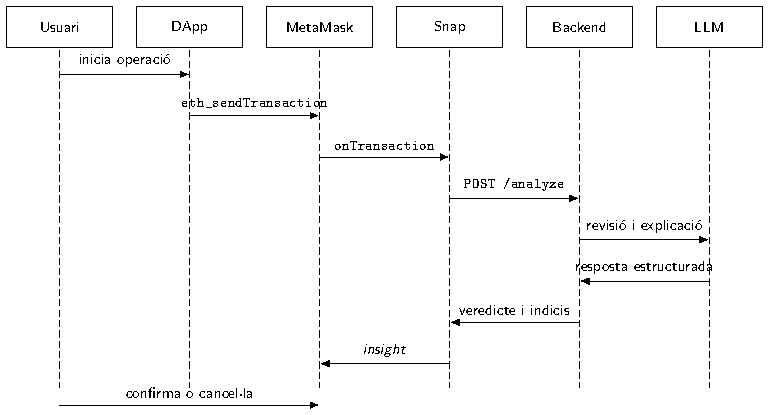
\includegraphics[width=\textwidth]{diagrams/render_sequence_general.pdf}
    \caption{Diagrama de seqüència dels casos CU1 i CU4: anàlisi prèvia i decisió final}
    \label{fig:seq-cu1-cu4}
\end{figure}

\paragraph{CU2 -- Anàlisi d'una aprovació ERC20.}
En aquest cas, la descodificació de \texttt{approve} permet identificar l'adreça autoritzada i la quantitat. Les regles combinen aquests camps amb el context local per distingir una revocació, un permís limitat o una aprovació pràcticament il·limitada.

\begin{figure}[H]
    \centering
    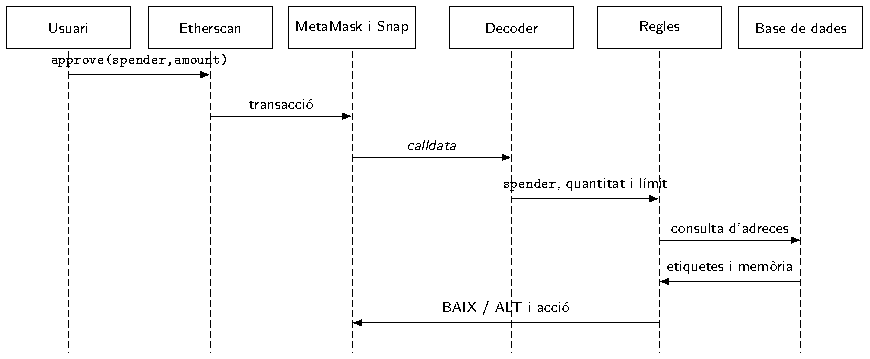
\includegraphics[width=\textwidth]{diagrams/render_sequence_erc20.pdf}
    \caption{Diagrama de seqüència del cas CU2: anàlisi d'una aprovació ERC20}
    \label{fig:seq-cu2}
\end{figure}

\paragraph{CU3 -- Anàlisi d'un permís global NFT.}
La interpretació del booleà \texttt{approved} és determinant: el valor \texttt{true} activa un permís global d'alt risc, mentre que \texttt{false} revoca l'autorització i produeix un resultat de risc baix.

\begin{figure}[H]
    \centering
    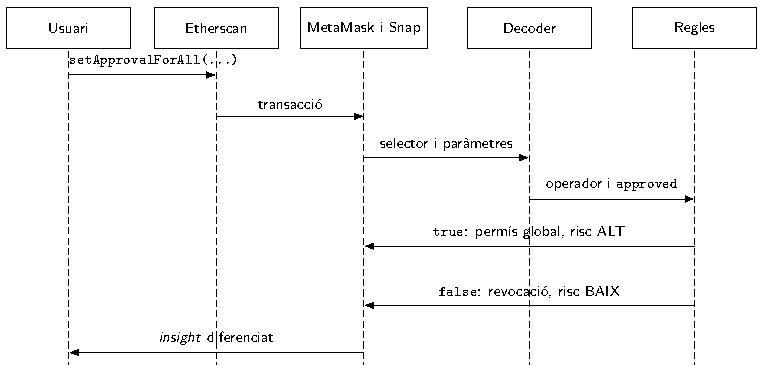
\includegraphics[width=0.92\textwidth]{diagrams/render_sequence_nft.pdf}
    \caption{Diagrama de seqüència del cas CU3: activació o revocació d'un permís global NFT}
    \label{fig:seq-cu3}
\end{figure}
